\begin{frame}
    \centering \href{https://twiki.cern.ch/twiki/bin/viewauth/AtlasProtected/JsvJetPhysicsValidation}{\Huge A tutorial to validation}
\end{frame}

\begin{frame}{Producing validation plots}
    \begin{block}{Why would you need any of this?}
        \begin{itemize}
            \item You want to make plots for validation
            \item You want a nice tool to easily make comparison plots from ntuples
            \item It is actually quite easy!
        \end{itemize}
    \end{block}
    \begin{block}{What are the requirements}
        \begin{itemize}
            \item A grid certificate (if you want to download files via rucio)
            \item Access to athena
            \item A gitlab account
        \end{itemize}
    \end{block}
\end{frame}
%
\begin{frame}{An example task}
   \begin{itemize}
       \item The details of the task are unimportant
       \item It shows good behaviour for an example
   \end{itemize}
   \begin{block}{Details of the task}
       \begin{itemize}
           \item Description: Validation of G4fix quasi-stable particle simulation for Run2 re-processing
           \item JIRA: https://its.cern.ch/jira/browse/ATLPHYSVAL-701
           \item Reference: valid1:valid1.410000.PowhegPythiaEvtGen\_P2012\_ttbar\_hdamp172p5\_nonallhad.merge.NTUP\_PHYSVAL.e4993\_s3634\_r12287\_p4360\_p3821
           \item Test: valid1:valid1.410000.PowhegPythiaEvtGen\_P2012\_ttbar\_hdamp172p5\_nonallhad.merge.NTUP\_PHYSVAL.e4993\_s3227\_s3653\_r12320\_p4360\_p3821
           \item \href{https://atlas-computing.web.cern.ch/atlas-computing/links/PhysValDir/JetEtMiss/exampleValidation_CKIRFEL/}{Webpage}
       \end{itemize}
   \end{block} 
\end{frame}
%
\begin{frame}[containsverbatim]{Setup}
        \begin{tcblisting}{listing only}
git clone ssh://git@gitlab.cern.ch:7999/ckirfel/jetphysvalidation.git
cd jetphysvalidation            
setupATLAS
lsetup 'rucio -w'
voms-proxy-init -voms atlas
        \end{tcblisting}
    Set up rucio as wrapper to avoid polluting environment
    This works only for CLI and no rucio APIs available
\end{frame}
%
\begin{frame}[containsverbatim]{Getting the files}
    \begin{tcblisting}{listing only}
        ./JetVal.sh
    \end{tcblisting}
    \centering 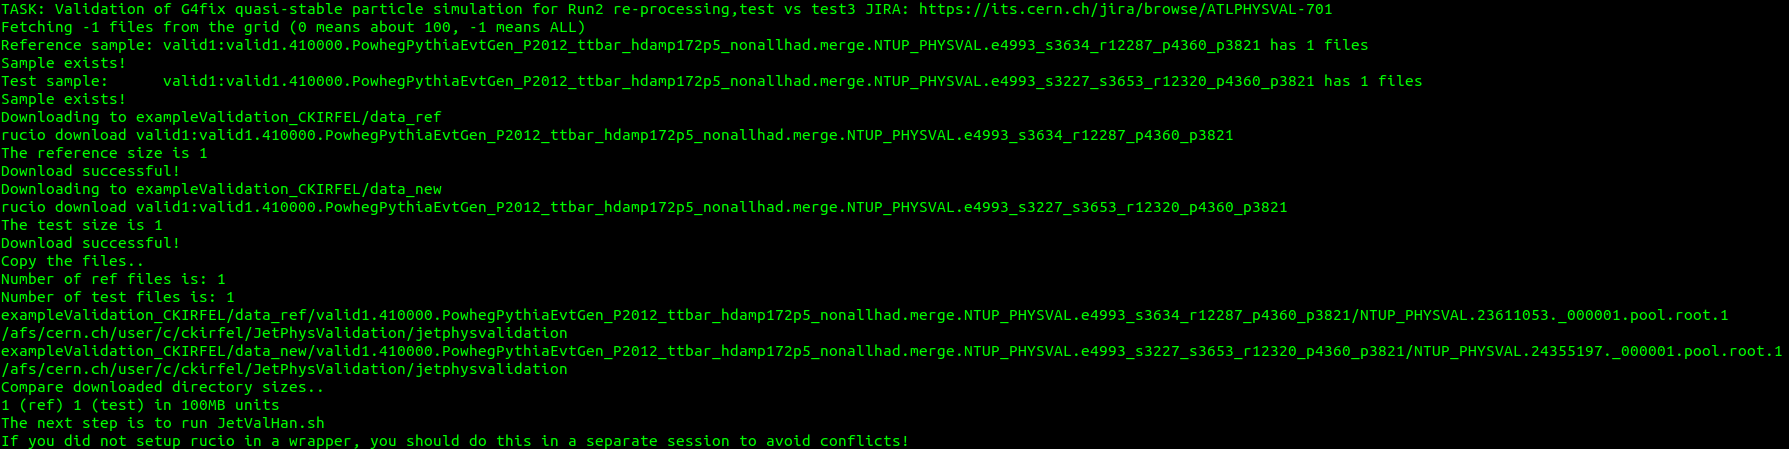
\includegraphics[width=\textwidth]{JetVal.png}    
\end{frame}
%
\begin{frame}[containsverbatim]{Making the comparison plots}
    \begin{tcblisting}{listing only}
        ./JetValHan.sh
    \end{tcblisting}
    \centering 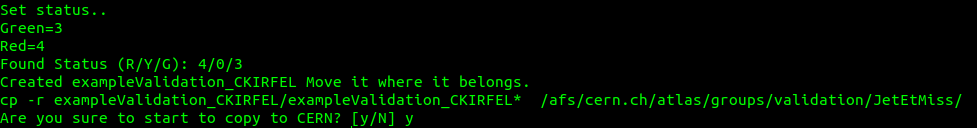
\includegraphics[width=\textwidth]{JetValHan.png}
\end{frame}
%
\begin{frame}{Checking the plots}
    \centering 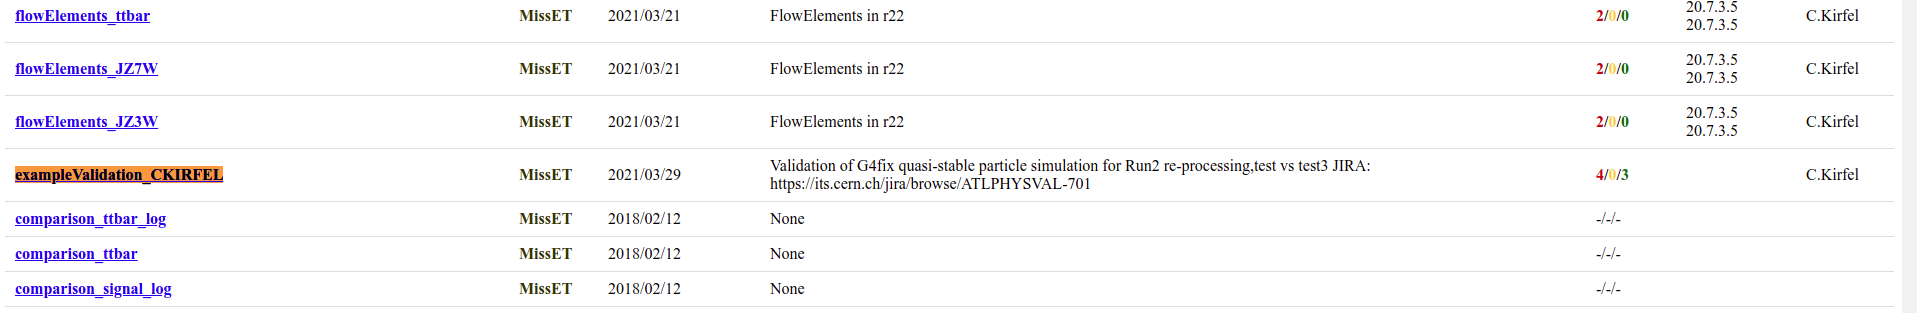
\includegraphics[width=\textwidth]{webpage.png}
    \href{https://atlas-computing.web.cern.ch/atlas-computing/links/PhysValDir/JetEtMiss/}{Validation webpage}
\end{frame}
%
\begin{frame}{Good agreement}
    \centering 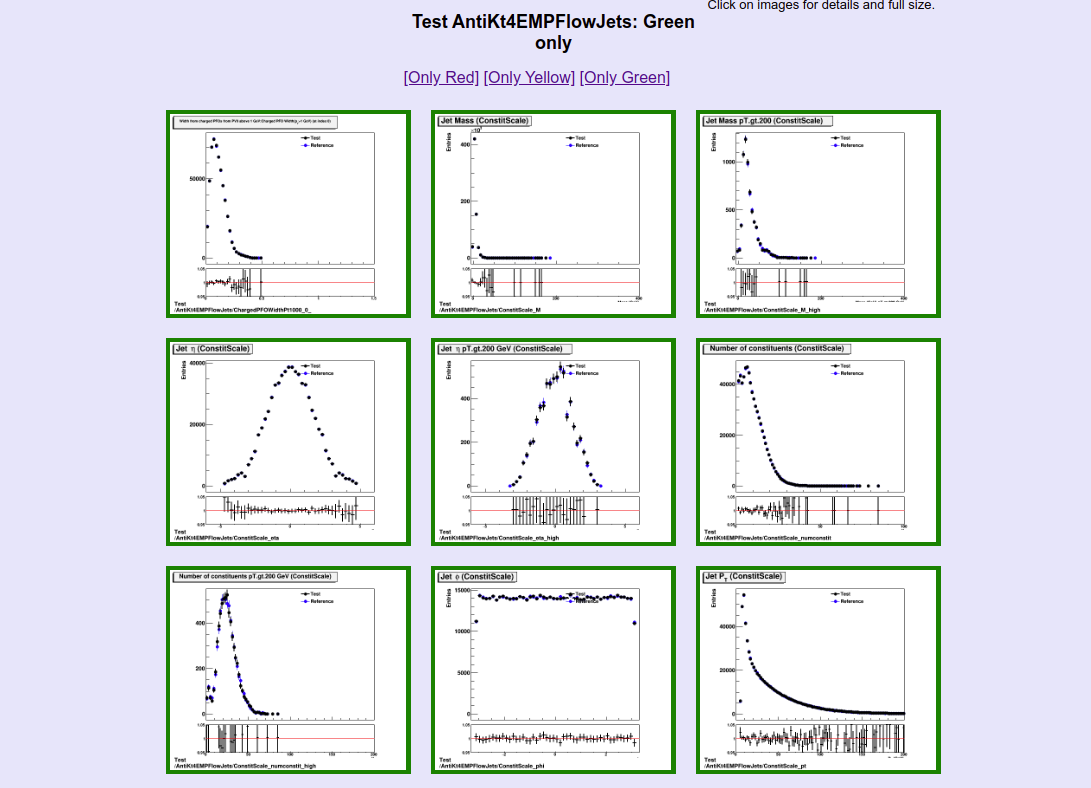
\includegraphics[width=\textwidth]{green.png}
\end{frame}
%
\begin{frame}{Medium agreement}
    \centering 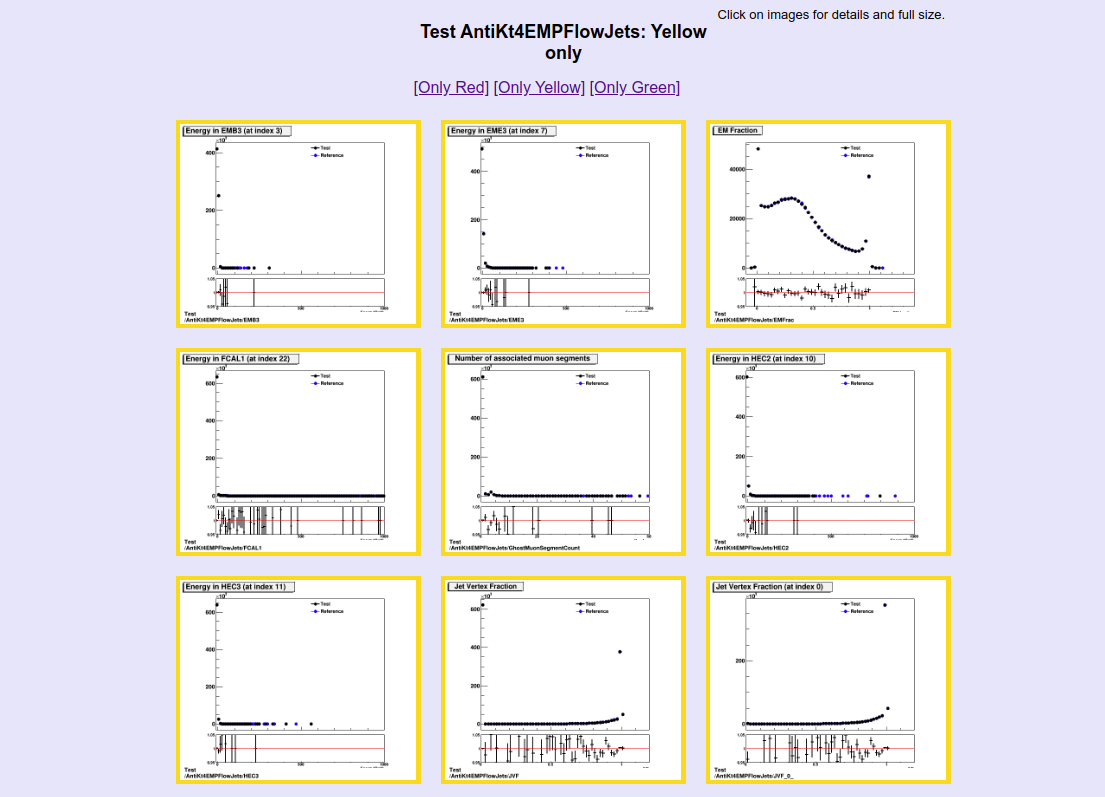
\includegraphics[width=\textwidth]{yellow.png}
\end{frame}
%
\begin{frame}{Bad agreement}
    \centering 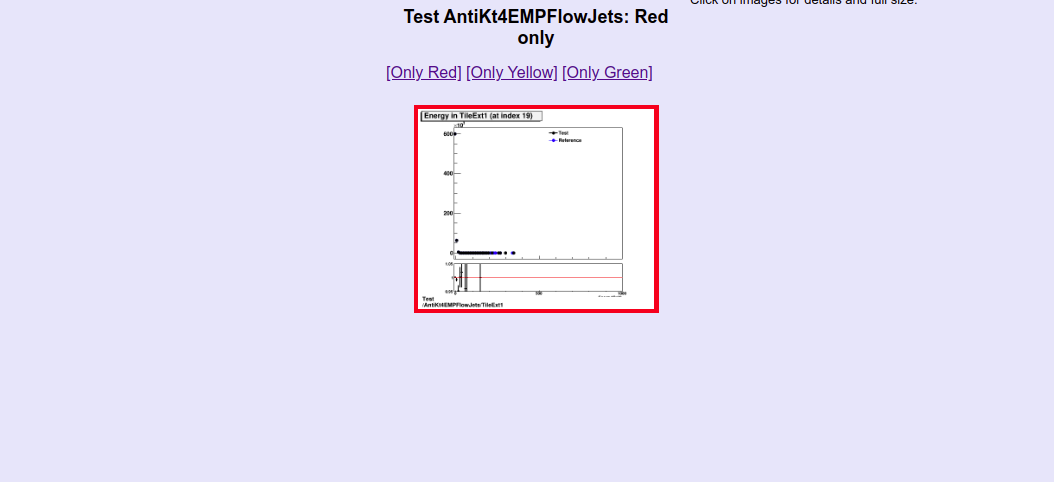
\includegraphics[width=\textwidth]{red.png}
\end{frame}
%
\begin{frame}{A plot in detail}
    \centering 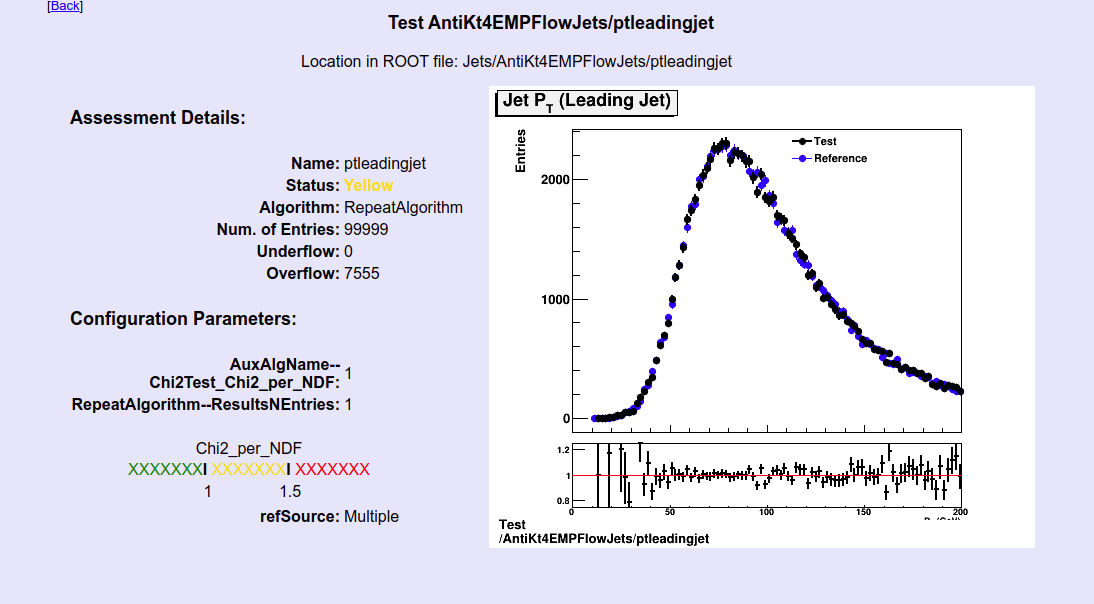
\includegraphics[width=\textwidth]{details.png}
\end{frame}
%
\begin{frame}{Checking the range}
    \centering 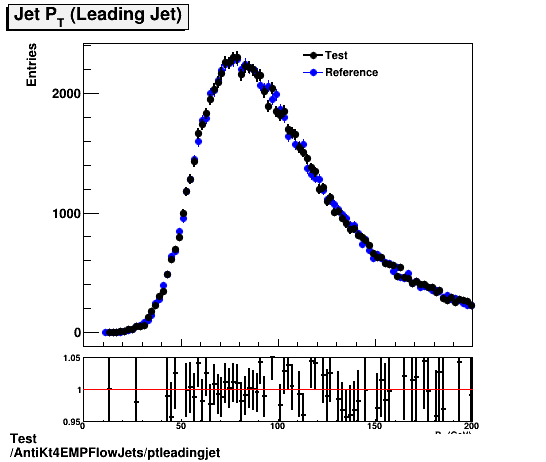
\includegraphics[width=0.7\textwidth]{smallRange.png}
\end{frame}
%
\begin{frame}{Checking the range}
    \centering 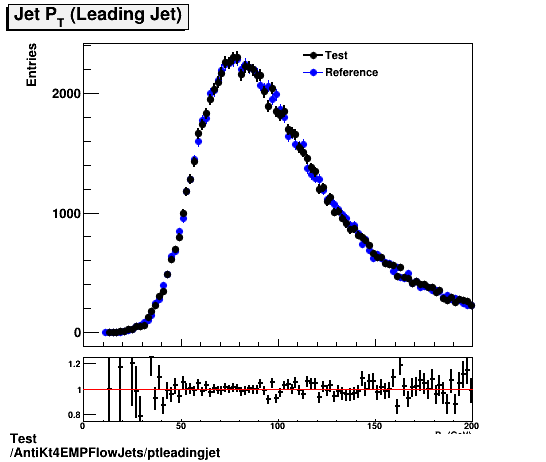
\includegraphics[width=0.7\textwidth]{largeRange.png}
\end{frame}

\begin{frame}[containsverbatim]{Utilized scripts 1: The web display}
    \begin{itemize}
        \item Tool to adjust the webdisplay
        \item Commonly used adjustments are arguments
        \item Some details have to be changed in the code
        \item \href{https://twiki.cern.ch/twiki/bin/viewauth/AtlasProtected/PhysValMonitoring}{TWiki}
    \end{itemize}
    \begin{tcblisting}{listing only}
        physval_make_web_display.py
        --reffile Reference:val_ref/output_ref.root 
        --outdir=$PROJECT --title Test val_new/output_new.root
        --startpath=Jets 
        --ratio --ratiorange=0.25 
        --normalize (or better scaleref)
    \end{tcblisting}
\end{frame}
%
\begin{frame}[containsverbatim]{Utilized scripts 2: The merger}
    \begin{itemize}
        \item Code used to merge multiple input files
    \end{itemize}
    \begin{tcblisting}{listing only}
        NTUPMerge_tf.py
        --inputNTUP_PHYSVALFile=$MERGE_REF 
        --AMITag="p3821" 
        --outputNTUP_PHYSVAL_MRGFile="output_ref.root"
    \end{tcblisting}
\end{frame}

%
\begin{frame}{Troubleshooting. Do not make my mistakes}
    \begin{itemize}
        \item You are using athena scripts, if you switched to a newer version that might have broken the code
        \item You might have used a local version of a script and forgot to switch back to the athena version
        \item Check that you have rights to push to the webpage
        \item You can always manually check that all files are in place and filled
        \item Check that you are not using the same file as test and ref by accident...
    \end{itemize}
\end{frame}